% Chapter 5

\chapter{Design and Implementation} % Main chapter title

\label{Chapter5} % For referencing the chapter elsewhere, use \ref{Chapter1} 

\lhead{Chapter 5. \emph{Design and Implementation}} % This is for the header on each page - perhaps a shortened title

\par 

\par 

% Chapter 5: Formal Model: Theoretical Development, Functional and Non-Functional Requirements, Implementation, Use cases, Testing

%----------------------------------------------------------------------------------------
\section{Functional Requirements}
%----------------------------------------------------------------------------------------

\par 

%----------------------------------------------------------------------------------------
\section{Non-Functional Requirements}
%----------------------------------------------------------------------------------------

\par 

%----------------------------------------------------------------------------------------
\section{Implementation}
%----------------------------------------------------------------------------------------

\par

%----------------------------------------------------------------------------------------
\section{Use cases}
%----------------------------------------------------------------------------------------

\par

%----------------------------------------------------------------------------------------
\section{Testing}
%----------------------------------------------------------------------------------------

\par

%----------------------------------------------------------------------------------------
\section{Results}
%----------------------------------------------------------------------------------------

\par For this section you will probably need some data to fit into other space - therefor just take a glance at your results and fit it into something - see figure \ref{fig:thesis-word-count.png}. 
% xkcd-python.png

\begin{figure}[H]
    \centering
    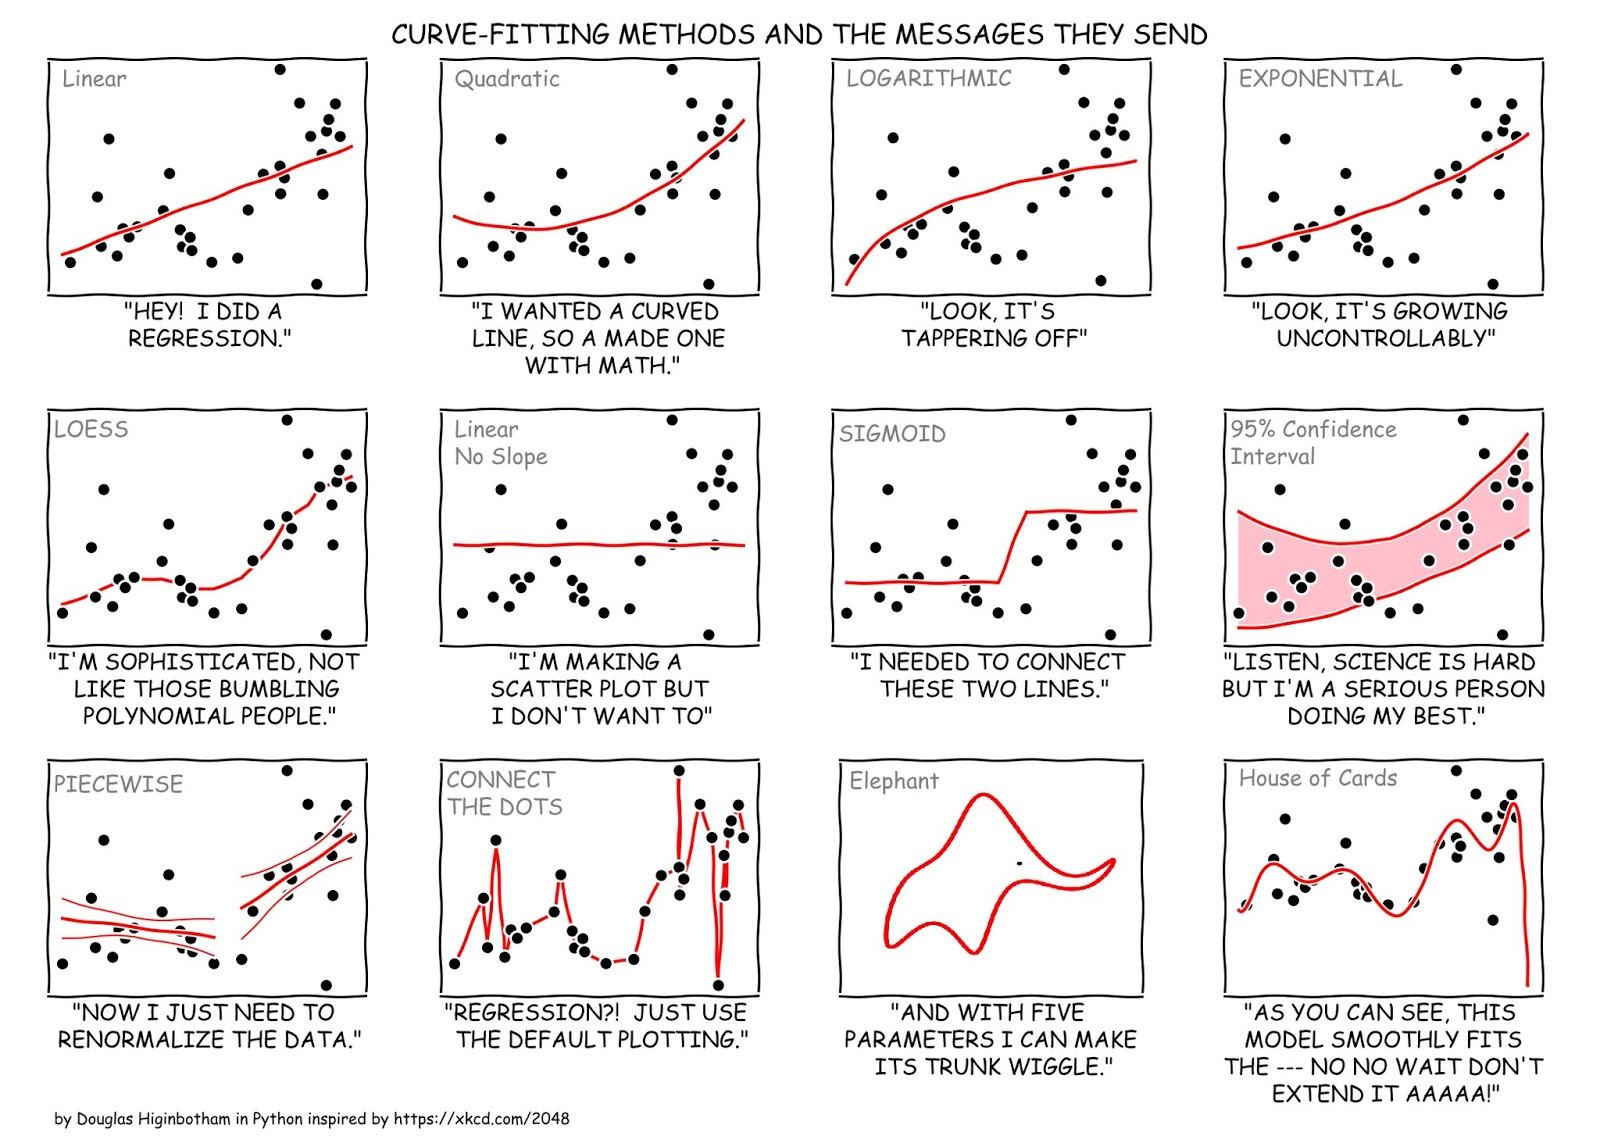
\includegraphics[scale=0.35]{Figures/xkcd-python.png}
    %\rule{35em}{0.5pt}
    \caption[Data fit]{Fit it}
    \label{fig:xkcd-python.png}
\end{figure}


%C\item Chapter 1: Introduction, Background, Motivation, Problem statement, Goals, Restrictions, Overview;
%C\item Chapter 2: Literature Survey and Background:  Research method, Methodology of Software Development, Literature review, Related Works
%C\item Chapter 3: Theoretical Foundations: Background Material, State of art, Internet of Things, Theory on hardware, Serverless architecture
%C\item Chapter 4: Protocol and systems(services and programs) used to build the system.
%C\item Chapter 5: Formal Model: Theoretical Development, Implementation / Use cases, Testing
%C\item Chapter 6: Algorithmic Considerations
%C\item Chapter 7: Implementation Issues, Results and Evaluation
%C\item Chapter 8: Discussion, Critical Appraisal, Conclusions
%C\item Chapter 9: Future Work 

%Chapter 1. Introduction & Overview
%Chapter 2. Literature Survey
%Chapter 3. Theoretical Foundations: Background Material
%Chapter 4. Formal Model: Theoretical Development (use additional chapters if necessary)
%Chapter 5. Algorithmic Considerations
%Chapter 6. Implementation Issues
%Chapter 7. Evaluation
%Chapter 8. Discussion & Critical Appraisal
%References
%Appendices
% Key Software listings
% Mechanical schematics
% Mathematical proofs